% 有线广播
% 有线广播.tex

\documentclass[12pt,UTF8]{ctexbook}

% 设置纸张信息。
\input{../../../../common/page}

% 设置字体，并解决显示难检字问题。
\xeCJKsetup{AutoFallBack=true}
% 注意：ctexbook类已默认设置SimSun为CJKrmdefault
% 以下设置用于确保字体回退和扩展字体可用
% 仅设置扩展字体以避免与默认设置冲突
\setCJKfamilyfont{hei}{SimHei}
\setCJKfamilyfont{kai}{KaiTi}

% 目录 chapter 级别加点（.）。
\usepackage{titletoc}
\titlecontents{chapter}[0pt]{\vspace{3mm}\bf\addvspace{2pt}\filright}{\contentspush{\thecontentslabel\hspace{0.8em}}}{}{\titlerule*[8pt]{.}\contentspage}

% 支持目录点击跳转
\usepackage[colorlinks,linkcolor=blue,citecolor=blue,urlcolor=blue]{hyperref}

% 设置 part 和 chapter 标题格式。
\ctexset{
	part/name= {第,卷},
	part/number={\chinese{part}},
	chapter/name={第,篇},
	chapter/number={\arabic{chapter}}
}

% 图片相关设置。
\usepackage{graphicx}
\graphicspath{{Images/}}

% 设置署名格式。
\newenvironment{shuming}{\hfill\zihao{4}}

% 注脚每页重新编号，避免编号过大。
\usepackage[perpage]{footmisc}

% 设置古文原文格式。
\newenvironment{yuanwen}{\bfseries\zihao{4}}

% 设置段落间距
\setlength{\parskip}{0.8em plus 0.2em minus 0.1em}

% 列表格式支持，列表项向右偏移。
\usepackage{enumitem}

\title{\heiti\zihao{0} 有线广播}
\author{}
\date{}

\begin{document}

\maketitle
\tableofcontents

\frontmatter
\chapter{前言}

本书系统地介绍了有线广播系统的基本原理、技术发展和实际应用。从早期的有线广播网络到现代的智能广播系统，全面覆盖了有线广播技术的各个方面。

本书适合广播工程师、通信技术人员、电子工程专业学生以及对广播技术感兴趣的读者阅读。通过本书的学习，读者可以掌握有线广播系统设计的基本原理，了解各种广播技术的优缺点，并能够进行实际的系统设计和维护工作。

\mainmatter

\part{有线广播基础理论}

\chapter{有线广播概述}

\section{有线广播的基本概念}

有线广播是一种通过有线传输介质（如电缆、双绞线等）将音频信号传送到多个接收终端的广播方式。与无线广播不同，有线广播具有信号稳定、抗干扰能力强、覆盖范围可控等特点。

近年来在我国广大的农村里，已普遍建立了有线广播收听网。它不仅可以用来指导生产和进行宣传教育，同时还能作为提高文化生活的工具。\textbf{实质上，有线广播是一座大功率的扩音机和许多扬声器的组合。}

\section{有线广播的发展历程}

有线广播技术的发展可以分为以下几个阶段：

\begin{itemize}[leftmargin=3.5em]
    \item \textbf{早期阶段}：使用电话线或专用线路传输音频信号
    \item \textbf{模拟阶段}：采用模拟信号传输，音质较好但传输距离有限
    \item \textbf{数字阶段}：采用数字信号传输，抗干扰能力强，支持多种业务
    \item \textbf{智能阶段}：结合物联网技术，实现智能化管理和控制
\end{itemize}

\chapter{有线广播系统组成}

\section{系统架构}

有线广播系统主要由以下几部分组成：

\begin{itemize}[leftmargin=3.5em]
    \item \textbf{音源设备}：麦克风、CD播放器、计算机等信号源
    \item \textbf{前置放大器}：对音频信号进行初步放大和处理
    \item \textbf{功率放大器}：将信号放大到足够功率驱动扬声器
    \item \textbf{传输线路}：电缆、双绞线、光纤等传输介质
    \item \textbf{终端设备}：扬声器、音箱等接收设备
    \item \textbf{控制系统}：实现分区控制、定时播放等功能
\end{itemize}

\section{传输介质}

常用的传输介质包括：

\begin{itemize}[leftmargin=3.5em]
    \item \textbf{双绞线}：成本低，适合短距离传输
    \item \textbf{同轴电缆}：抗干扰能力强，传输距离较远
    \item \textbf{光纤}：传输距离远，带宽大，适合大型系统
\end{itemize}

\section{扩音机与扬声器}

扩音机的主要任务是把语言和音乐的信号加以放大。图\ref{fig:amplifier-diagram}所示的是扩音机各部分的方块图。由送话器或拾音器把声音信号变成音频（低频）电压，经扩音机把音频电压放大以推动扬声器发出具有足够强度的声音。

来自送话器或拾音器的音频电压是非常微弱的，必须经过多级电压放大，最后经过功率放大，才能获得足够大的输出功率，来推动许多只扬声器。对于有收音设备的扩音机，可以直接收听电台的广播。

在有线广播中，扬声器是供用户使用的主要设备，连接得是否合适，不仅直接影响收听质量，而且还会影响整个广播网路和其他用户。

\begin{figure}[H]
	\centering
	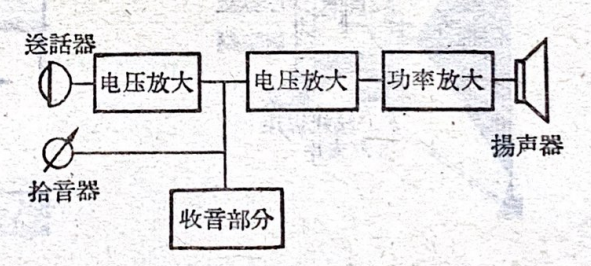
\includegraphics[width=0.8\linewidth]{amplifier-diagram.png}
	\caption{扩音机示意图}
	\label{fig:amplifier-diagram}
\end{figure}

\subsection{扬声器的工作原理}

扬声器是一种电声转换元件，依靠它把音频电流还原成声音，也就是把电磁能转换成声能，使我们可以听到广播的语言或音乐。各种扬声器的工作原理基本上是相同的，现在就以农村中用得最多的舌簧扬声器为例，来说明它是怎样把电磁能转变成声音的。

在用软铁制成的扁平舌簧的外面套一个线圈，放在永久磁铁的两只极靴的中间。当音频电流经过线圈时，舌簧被磁化。如果某一时刻电流方向如图中所示，根据右手拇指法则，这时舌簧的右端则为南极，左端为北极，它受到永久磁场的作用，右端将被吸引向上，左端向下，动作的方向如图中箭头所示。当电流方向改变时，舌簧动作的方向也就相反。这样舌簧就将随着线圈中所通过的音频电流的变化规律而来回地振动。舌簧又通过传动杠杆与纸盆相连，于是纸盆也就产生与音频电流相应的振动，从而激动空气成为声音。

\begin{figure}[H]
	\centering
	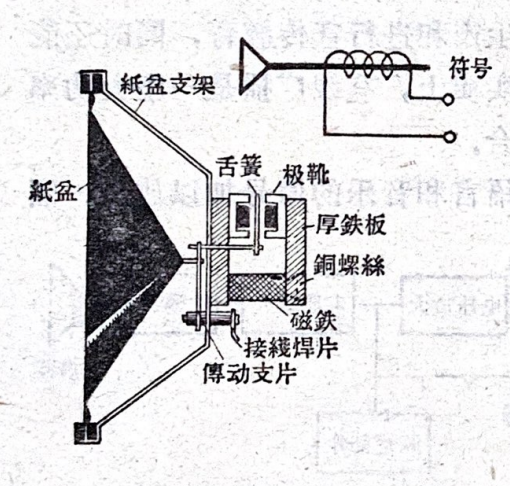
\includegraphics[width=0.7\linewidth]{reed-speaker-structure.png}
	\caption{舌簧扬声器的结构图}
	\label{fig:reed-speaker-structure}
\end{figure}

\begin{figure}[H]
	\centering
	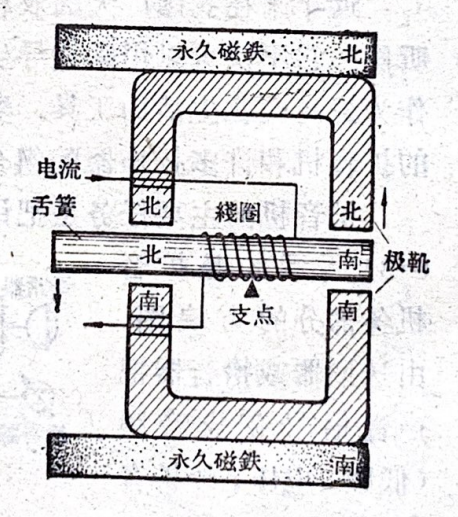
\includegraphics[width=0.7\linewidth]{reed-speaker-principle.png}
	\caption{舌簧扬声器的工作原理图}
	\label{fig:reed-speaker-principle}
\end{figure}

\chapter{有线广播技术原理}

\section{信号传输原理}

有线广播的信号传输基于模拟或数字信号处理技术：

\begin{itemize}[leftmargin=3.5em]
    \item \textbf{模拟传输}：直接传输音频信号的模拟波形
    \item \textbf{数字传输}：将音频信号数字化后传输，具有更好的抗干扰性能
\end{itemize}

\section{功率放大技术}

功率放大器是有线广播系统的核心设备，其性能直接影响广播质量。主要技术指标包括：

\begin{itemize}[leftmargin=3.5em]
    \item \textbf{输出功率}：决定系统覆盖范围和音量大小
    \item \textbf{频率响应}：影响音质的保真度
    \item \textbf{失真度}：反映信号还原的准确性
    \item \textbf{效率}：影响能耗和散热设计
\end{itemize}

\backmatter

\end{document}
